%----------------------------------------------------------------------------------------
%	Software
%----------------------------------------------------------------------------------------

\chapter{Software Components}

\section{Embedded Software}
The embedded software is responsible for taking the electrical signal provided by the hardware, and converting it to to a weight. When a stable weight measurement is taken it is  sent to the backend and shown consistently on the display. The LED display provides an easy and use friendly way to view the current weight of the scale. This display will give the user confidence the scale is working and show whether the weight is fluctuating. Sustainability is also considered by providing a low power sleep mode to reduce energy consumption. This sleep mode will be automatically entered when the weight is no longer changing and woken up from when a new weight is detected. 

The embedded software ensures accurate results of the scales by filtering the received voltage signals using averaging and outlier removal. Firstly a measurement of the ground voltage is taken, this is to get an approximation of the ADC offset which is subtracted from the final result to gain a higher accuracy. Multiple sets of averages of the voltage signal from the output of the Wheatstone bridge are then taken so that our application can update the display without long pauses in between updates. Once we have taken a specified number of averages, the highest and lowest samples we received are checked. If the difference between them is less than a configurable threshold value, we will determine that the weight is moving and not stable. Through testing, we determined this threshold to be 0.3 kgs which stayed accurate for different-sized weights. To determine the conversion between voltage and weight the scale was calibrated using known weights. A linear equation was derived to get a relationship between known weights and the ADC output, using this information. This equation was calibrated for maximum accuracy for all weights between 0-25 kg. Overall, the processing done in the embedded software to the weight signal is complex and robust to maximise the accuracy of the scale’s measured weight. Figure  \ref{fig:weight_acc} shows how the scale remains accurate over the whole weight range. The worst error measured was 0.2 kg. 

\begin{figure}[!ht]
	\centering
	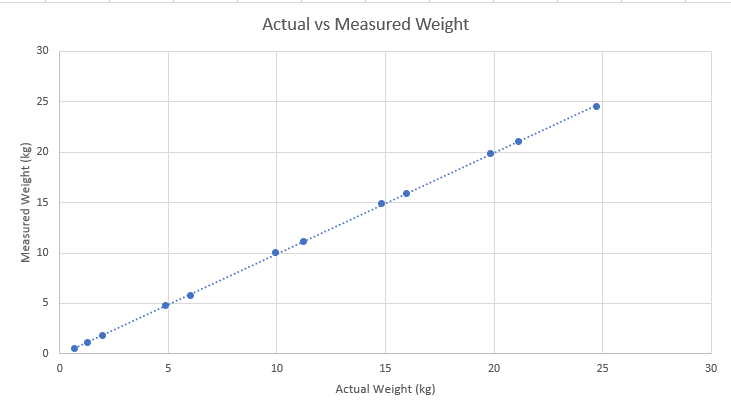
\includegraphics[scale=0.7]{weight-acc.png}
	\caption{Weight Accuracy Validation Graph}
	\label{fig:weight_acc}
\end{figure}

Once the weight has been determined stable, by having a weight reading within the required threshold the weight is sent to the backend of the software, the measurement LED turns on and the display flashes the final weight. After the display flashes, it will show the stable weight until the weight is removed from the scale or it goes to sleep. The flow of the embedded software is shown in Figure \ref{fig:emd_flow_chart} as well as the connections to the hardware and software backend.

Sleep was implemented in the embedded software to save power when the scale is not being used. If a weight on the scale has not been changing for seven seconds, then the embedded software will put itself to sleep. It will then wake up every two seconds and read the current weight on the scale. If the current weight has changed by a configurable threshold since the last wake up measurement, then the scale will wake up, if not it will go back to sleep. When in sleep mode, the system will turn all LEDs and the LED display off. It will initialise the wifi module, and turn off other unused clocks like the USB and ADC clocks and disable the external oscillator. Turning off these modules will save considerable amounts of power ensuring that SPCA staff do not need to be constantly changing the batteries of the scale. Thus, to the user it will continue to just ‘work’ making it easier and simple to use. 

The scales communicate with the backend via TCP over HTTP. Upon wake up, the scales asynchronously connect to the wifi in the background, this frees up the processor to start processing weight samples as soon as possible. Once a stable weight has been measured a TCP connection is initialised and connection to the backend is made. The connection and the sending of data to the backend is also done in the background, this provides a smoother user experience to SPCA staff as there are no long blocking pauses when connecting or   sending to the backend. Once a response has been received from the backend indicating the weight has been added then then the TCP connection is closed. Further, by displaying the real-time weight on the LED display instead of sending it constantly over wifi, it reduces the noise in the hardware weight signal to further increase accuracy.

\begin{figure}[!ht]
	\centering
	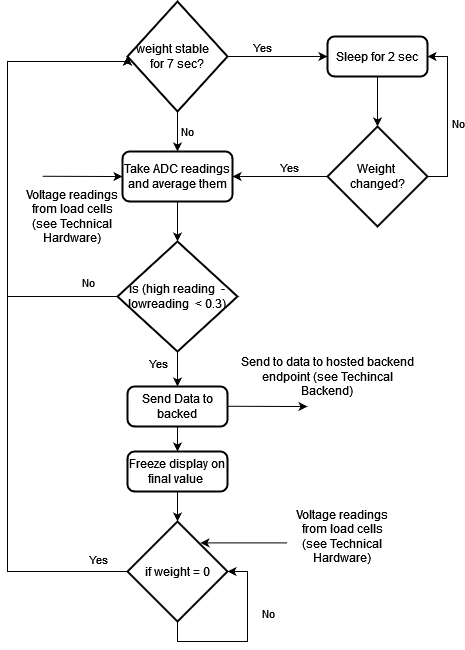
\includegraphics[scale=0.4]{emd-flow-chart.png}
	\caption{Embedded Software Flow Chart}
	\label{fig:emd_flow_chart}
\end{figure}



\section{Backend}
The backend API endpoints serve the business logic for the application's frontend and communicate with the database for data manipulation and storage. The technology we used for the backend is .NET 6 framework for all the API endpoints and SQLite for the relational database. We used .NET because it contains all the authentication, authorisation, endpoint, and database functionalities needed for the backend architecture. This also reduces the dependencies required to build the backend since no external packages are needed. All endpoints are hosted on MyAsp.net with HTTPS except for the endpoint communicating between the hardware and the backend, which is implemented in HTTP for simplicity, and the general data flow diagram is shown in Figure \ref{fig:general_data_flow}.


\begin{figure}[!ht]
	\centering
	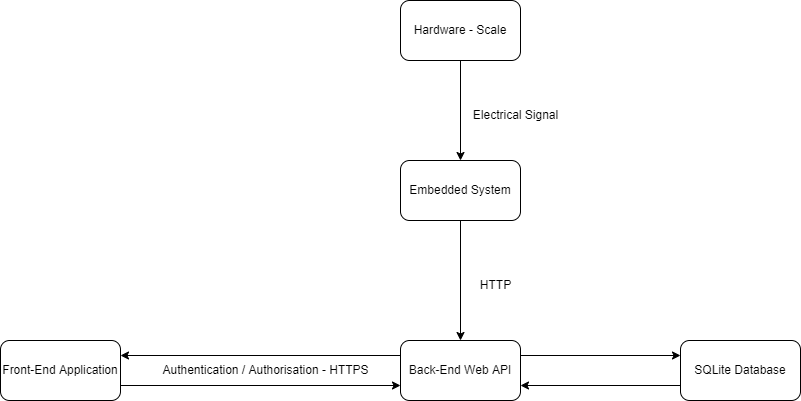
\includegraphics[scale=0.5]{general_data_flow.png}
	\caption{General Data Flow diagram of the Application}
	\label{fig:general_data_flow}
\end{figure}

Regarding database schema, we have seven tables in the database schema, namely Users, Messages, Centres, Dogs, Weights, Scales, and Requests as shown in Figure \ref{fig:database_schema}.  

\begin{figure}[!ht]
	\centering
	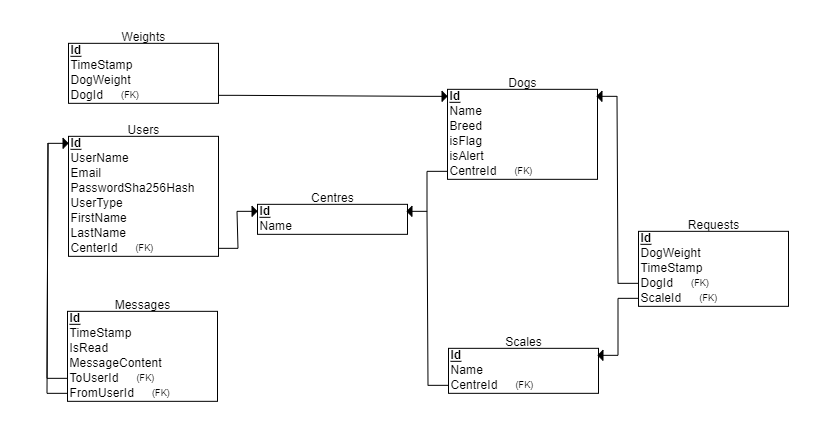
\includegraphics[scale=0.8]{database_schema.png}
	\caption{Database Schema for the Application}
	\label{fig:database_schema}
\end{figure}

The User table has the record of each user, including their username for login and the sha256 hash of their password. The reason that the hash of the password is used instead of the plain text password is that in case the database is compromised, user login is safe as the sha256 serves as a one-way function, so there is no way to retrieve the original password from the hash saved in the database. Other personal information is also stored in the entries for each user in the Users Table.
The Centers and Scales tables serve the simple purpose of providing matching names with different centre ID or scale ID.
The Messages table has all the records of messages for all users. The frontend application can query with the Endpoint to retrieve all chat history relating to a particular user through the FromUserId and ToUserId attributes in the database.
The Dogs table holds information for each dog, including centerId, name, bread, isFlag, and isAlert toggle indicator for the frontend application display. The Weights table holds each weight record for various dogs, which may have 0 or many weight records.
The Request table serves as temporary data storage for incoming weight elicited from the scale after matching with the dog information supplied from the frontend application. The corresponding entry in this table is deleted either by exceeding the two-second expiry time or after being saved by the user from the frontend application. This deleted entry is replaced with a new permanent entry in the Weights table. This method prevents spam data from affecting the permanent entries in the database and measurements affected by system crashes or network outages.


The final API endpoints implemented in this project are shown in Figure \ref{fig:api_endpoints_list} from Appendix \ref{appendix-backend}. The main categories of the endpoints are User related, Dog related, Chat related, and Util related (including Misc. functions and statistics). All endpoints use HTTPS for communication except one endpoint (/dog/addWeightFromScale) that uses HTTP to communicate from the scale hardware to backend for simplicity.


The main backend business functionalities of the application are to save the weight of a dog into the database, save chat messages, and send message notifications to users through emails.

The frontend user must specify that they are trying to weigh a dog before the backend saves the incoming weight. This ensures that the correct dog and scale are used to measure the dog's weight. We store the weight sent from the scale in a temporary request table for the reasons previously mentioned. The user can save the weight displayed on the frontend to the database via a confirmation button. Upon confirmation, the backend will receive the data through a POST request. User confirmation is essential to prevent incorrect data being saved to the database. The user can cancel the weight measurement operation, which drops the weight information recorded from the scale.

Chat messaging is another main area of business logic. Chat messages are sent to the database and retrieved on the client side. This is so that we can display chat message history on the frontend. Notifying the recipient of incoming messages is vital if the information is time sensitive. Thus, we decided to send notifications via email as most employees check their work emails, and emails have a notification system.

For authorisation and authentication, we have protected our endpoints with basic authentication, a form of bearer authentication that is popular and secure. On top of this, we have set up three different user roles: admin, vets, and volunteers. Admins have the highest access, while the other user roles have limited access to all API endpoints. Endpoint access is defined in the API endpoints based on user roles. By setting the access level of different user roles, we have closely followed the requirements of the project and prevented any usage and data abuse from happening.

Regarding secured HTTP, we have set up all the endpoints to use HTTPS for communication except one endpoint (/dog/addWeightFromScale) that uses HTTP to communicate from the scale hardware to backend for simplicity. HTTPS encrypts sensitive information during an HTTP request’s transmission. Encryption means that malicious observers cannot observe the data being sent [1].

Overall, the project's backend has been implemented with the requirements in mind and coded modularly to allow easy future expansion.


\section{Frontend}
Two frontend applications have been developed, a web platform and a mobile platform. These communicate with the backend to send and receive data, and expose a range of functionalities to the users. Both applications have the same main functionality, and the web platform also allows data to be exported to be used in applications such as Microsoft Excel. 

In order to allow for future expansions, the codebases have been built using clean code principles and are easily scalable. GitHub is used for version control, and the code is written in well-known languages to allow for future developers to easily contribute to the product. The web platform is written in React.js, and uses two popular and well-maintained libraries: Material UI (MUI) for visual components, and Axios to enable efficient https communication with the backend. The mobile application is written in Android Studio, using Java and xml. The OkHttp3 library is used to handle HTTP requests that allow the frontend and backend to communicate. Android Studio is equipped with a suite of tools that allowed us to design, build and test the application, which allowed for a fast development cycle. 

The applications are designed to be intuitive and user-friendly in order to lower the barriers to use. Styling and functionality across the web and mobile applications are consistent to make the brand cohesive and to reduce the learning curve for new users. A blue colour theme is used to be consonant with the SPCA branding. The light and clean design is fitting for a professional website, and is not intimidating for users who are not technically proficient. All text is large, high-contrast and in a sans-serif font to support any employees with impaired vision. All pages are accessible from the navigation bar in both applications, ensuring eacy and clear navigation. The applications require a wi-fi connection to function due to the cloud-based backend, however large amounts of data or files are not used so that the applications are usable even with a weak connection. We integrate Te Tiriti O Waitangi throughout the application and development team. Our applications contain translations in Te Reo Māori, and we designed our platform to be cohesive with Māori tikanga. We acknowledge the whakapāpā of the SPCA, through features such as showing centre data rather than each dog in a siloed perspective, and through the chat feature. 

In order to achieve cross-platform synchronisation, all data is stored in the backend. This means that any changes made on the mobile platform will be instantly viewable from the web platform. Because of this, the user can take weight measurements on their phone and instantly view this data on their computer. 

The login page connects to the backend to authenticate the user. Each user will belong to one of three access levels: volunteer, vet or admin. Only administrators can access user information and all dog information, which helps to protect data privacy. Other users can only access their own data, and dogs that are housed at the centre where they work. Key data flows between the backend and frontend for the login page are shown in figure \ref{fig:mob_login}. 

\begin{figure}[!ht]
    \centering
    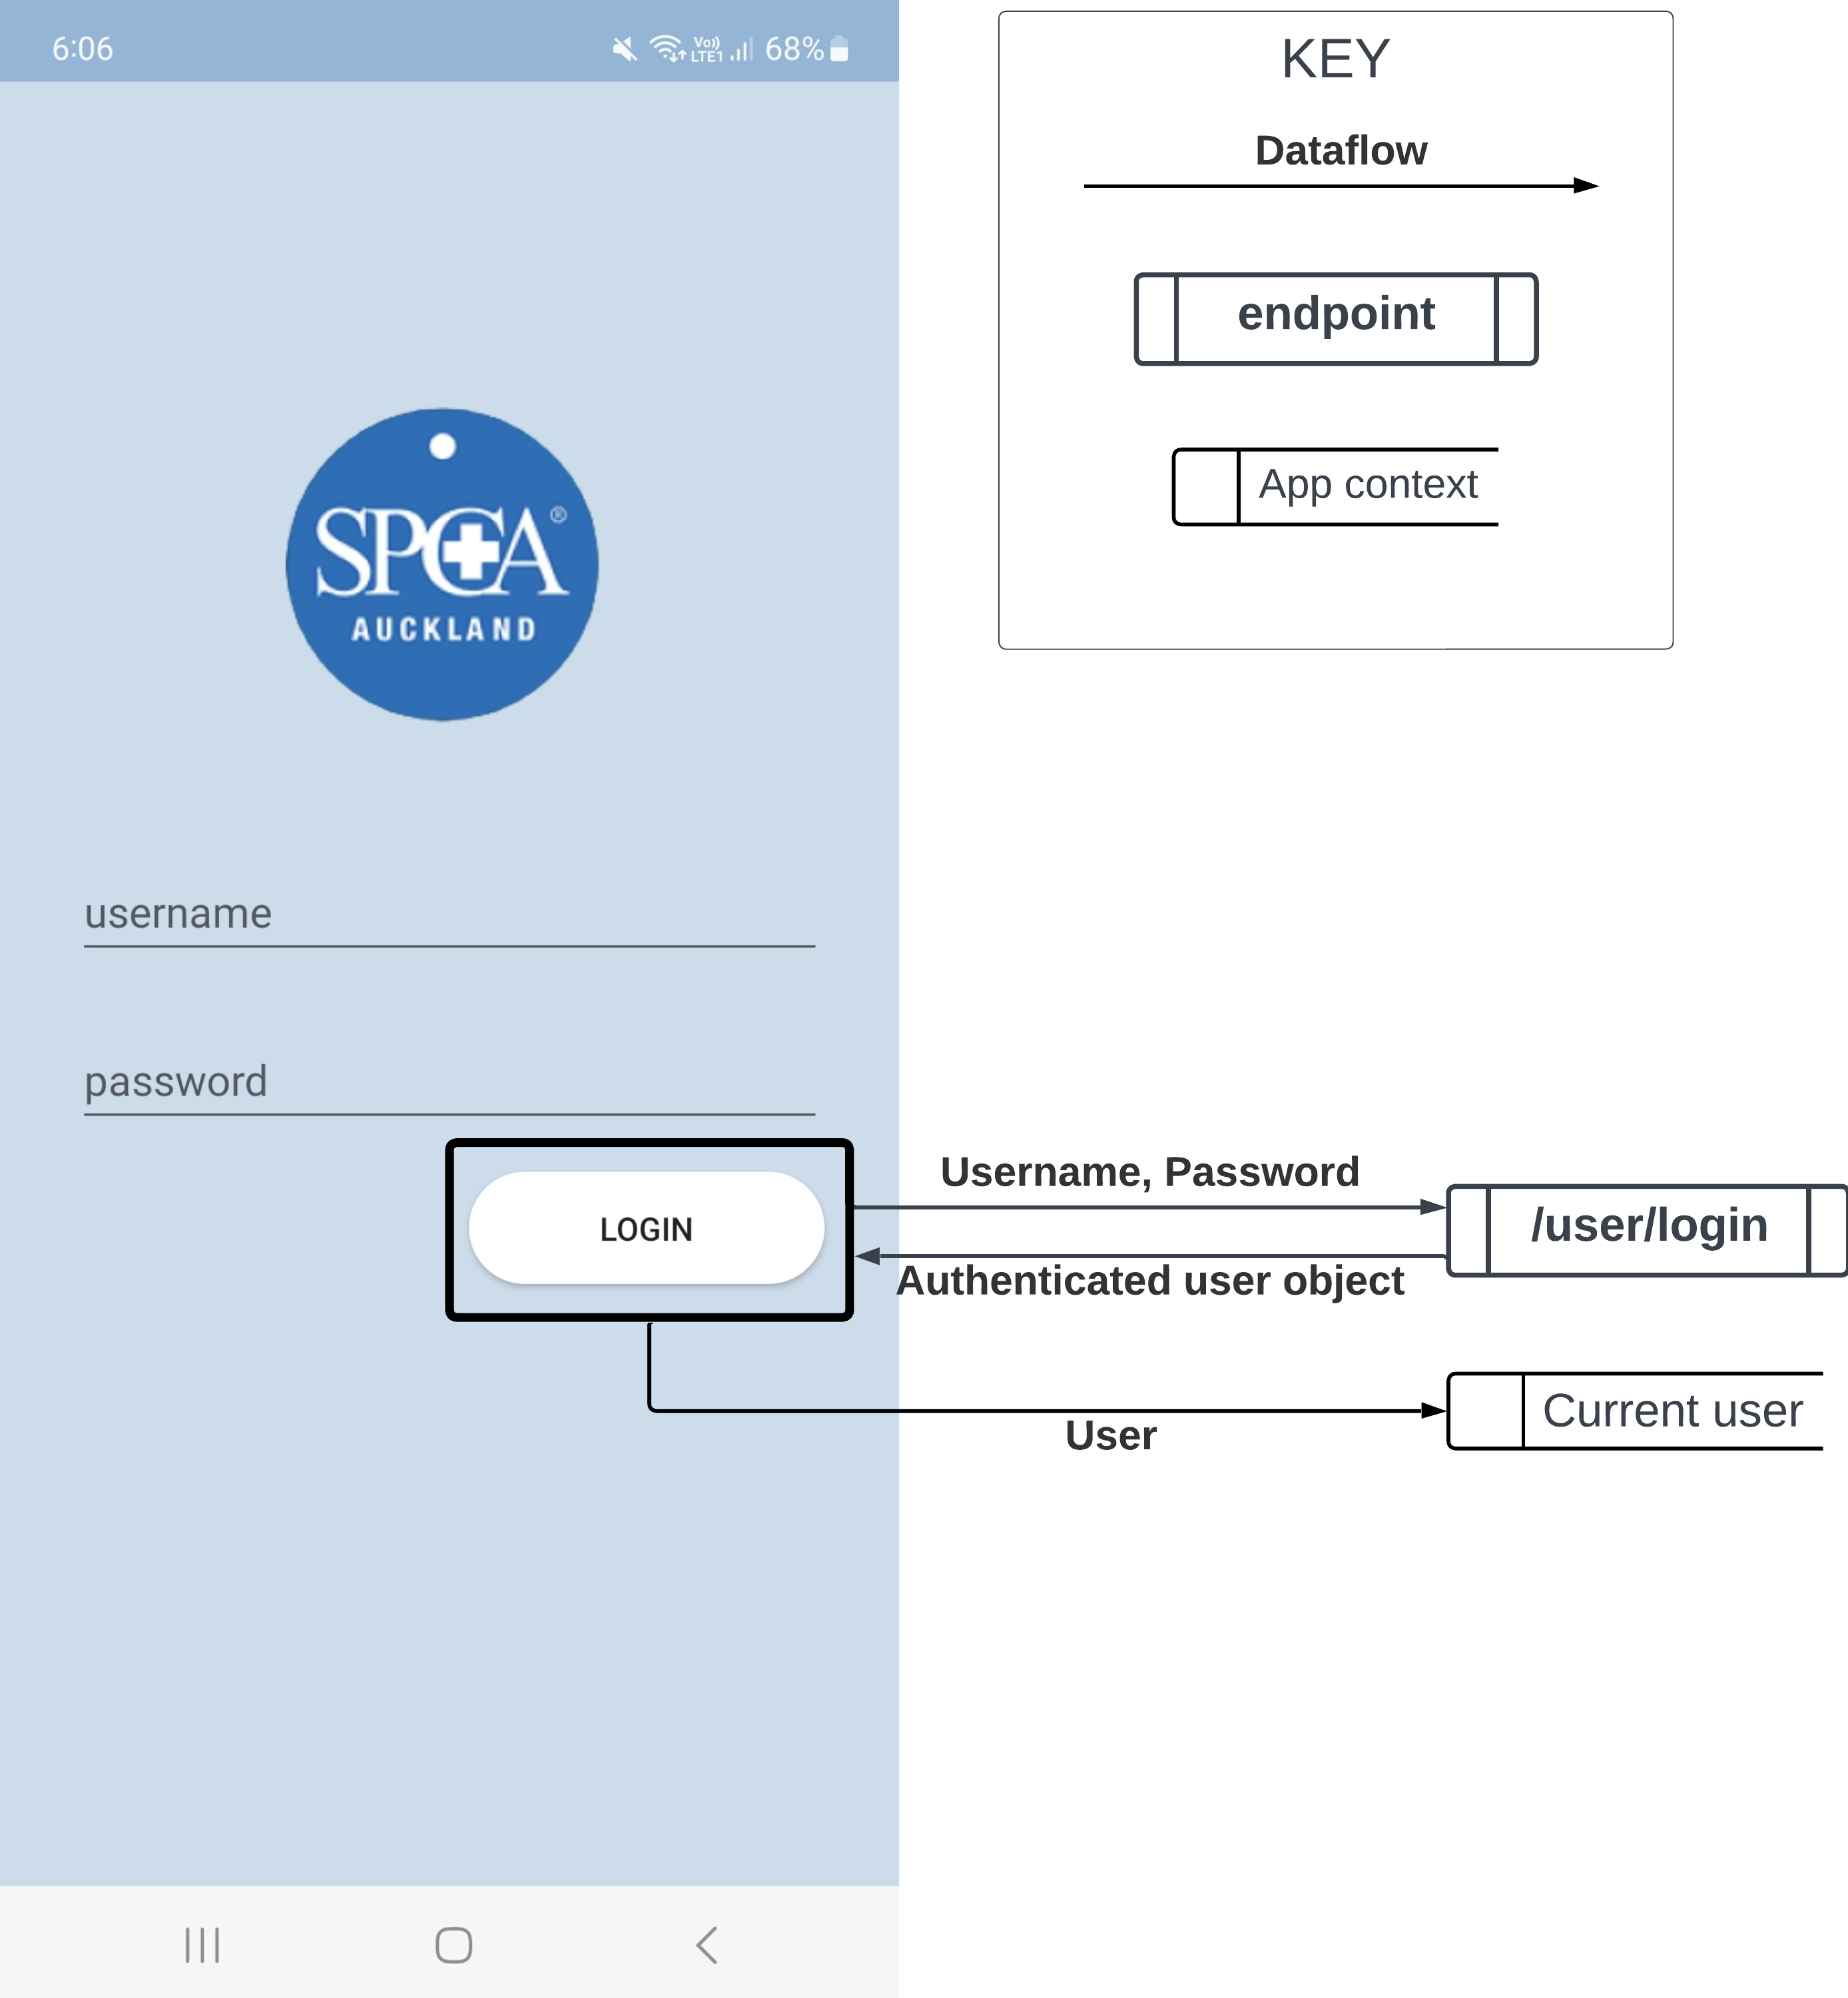
\includegraphics[scale=0.05]{login_flow.png}
    \caption{Login screen and data flow}
    \label{fig:mob_login}
\end{figure}

The home page displays a list of dogs that the user can access, as seen in figure \ref{fig:mob_home}. The primary task that the user will conduct is weighing a dog, so having this accessible from the homepage streamlines the user's process. This data is fetched from the backend so that it is always the latest version available. The mobile version shows a more simplified view, with only limited filtering available. We expect that the user will use the mobile application primarily to search for the dog that they want to weigh. The web application will be used for more analysis, so the table is more customisable with filters, sorting, customisable columns and data exporting functionality as seen in figure \ref{fig:web_home}. All users are able to create a new dog, as we expect that volunteers will handle some of the intake work at the SPCA. By clicking 'view', the user can see the full details of the dog. The user can easily navigate between all screens using the navigation bar, which contains clear icons and text to help the user navigate quickly and easily.

\begin{figure}[!ht]
    \centering
    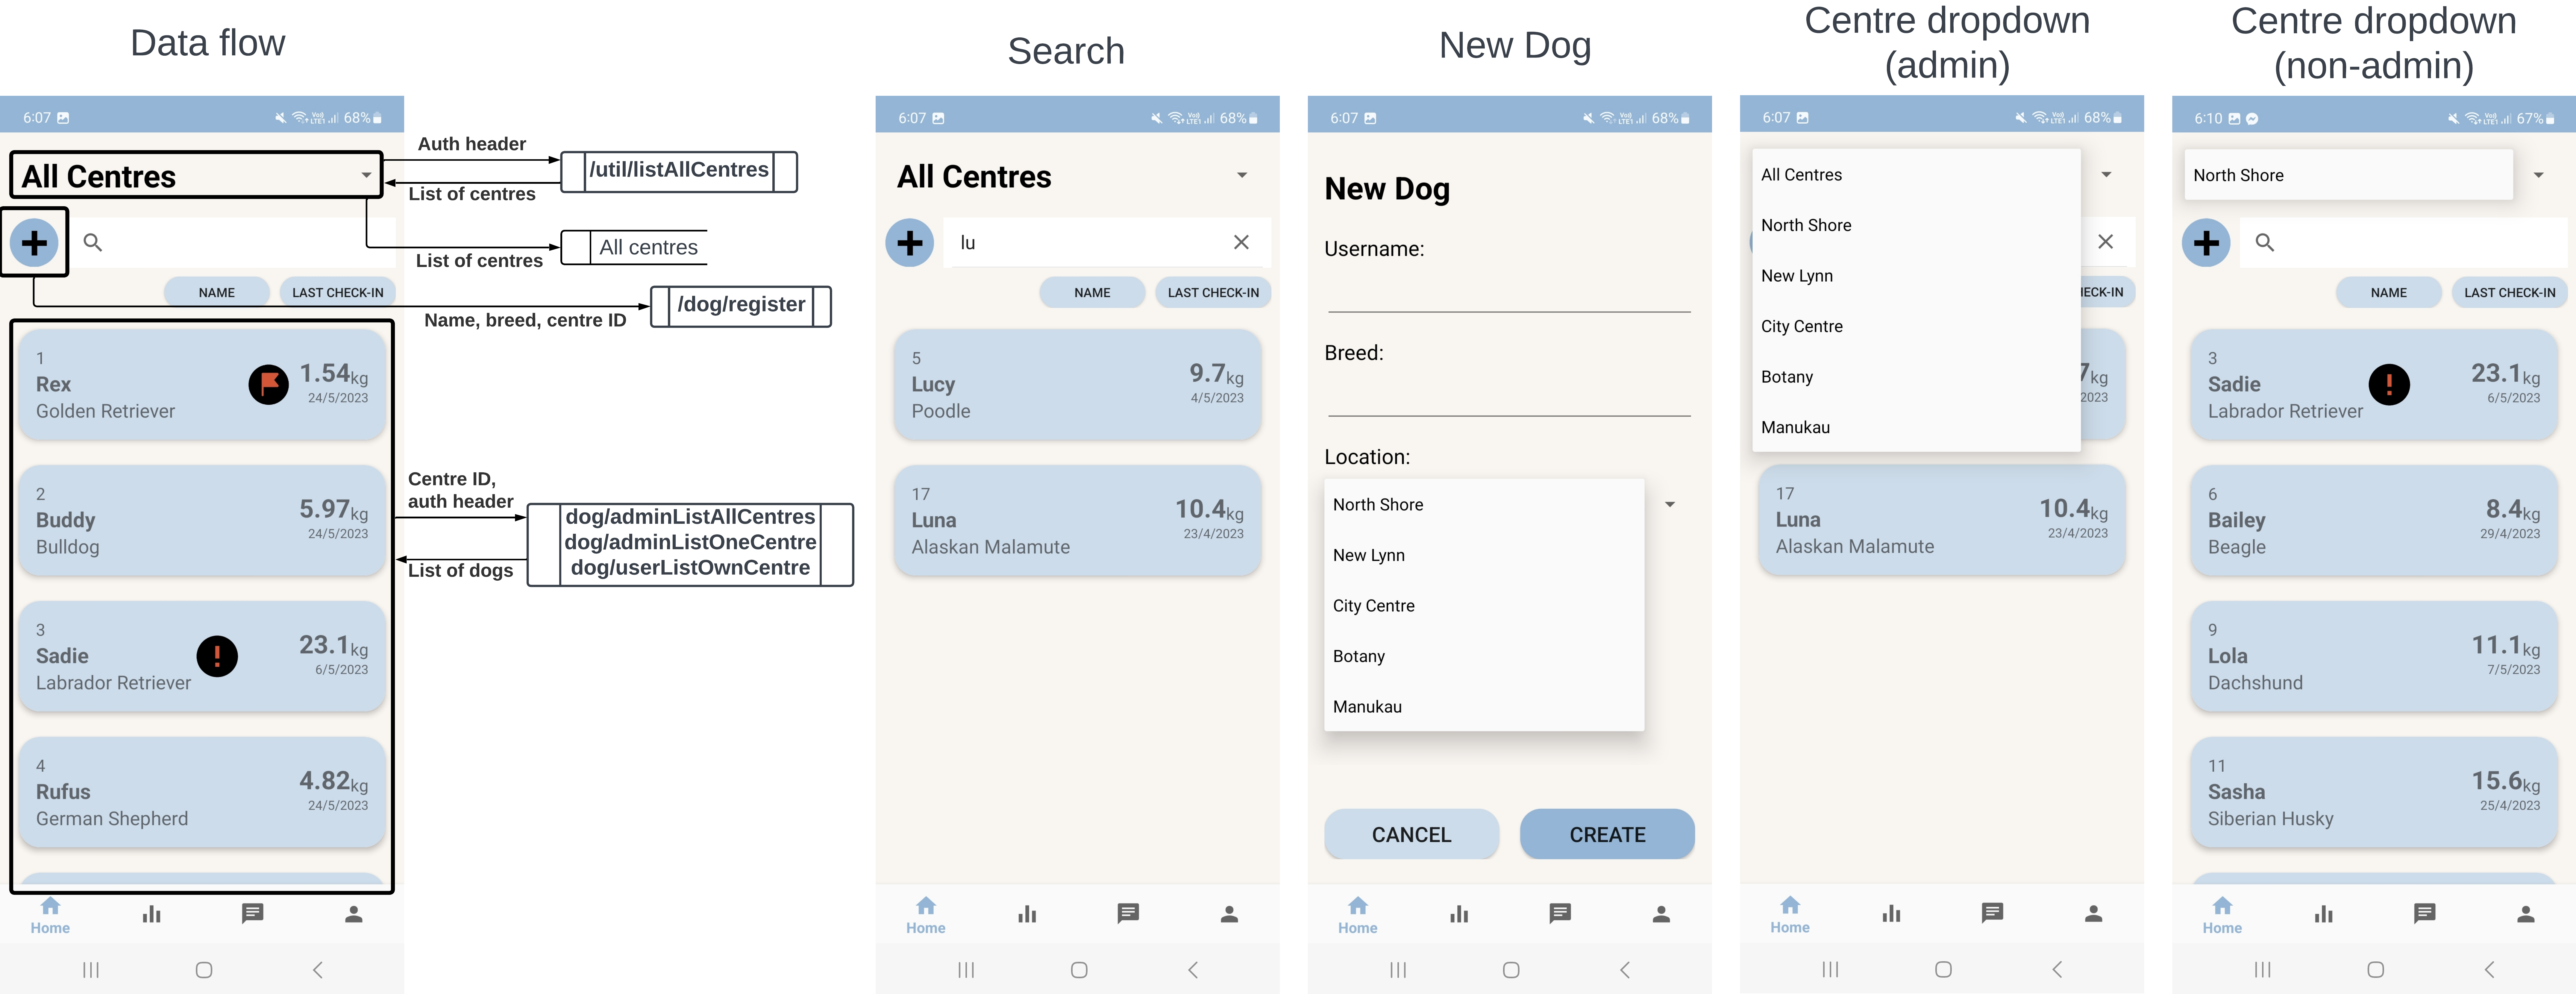
\includegraphics[scale=0.05]{home_flow.png}
    \caption{Mobile home screens and data flow}
    \label{fig:mob_home}
\end{figure}

\begin{figure}[!ht]
    \centering
    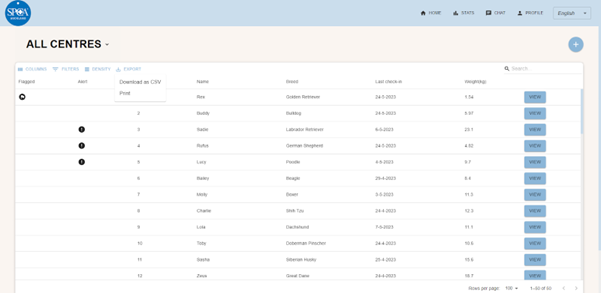
\includegraphics[scale=0.5]{home_web.png}
    \caption{Web home screen with additional export options}
    \label{fig:web_home}
\end{figure}

The dog page shows the key information of the dog, and allows the user to edit this information. Vets and admins can toggle the ‘flagged’ and ‘alert’ status or a dog. Flagged indicates that the dog is undergoing troubling weight change, and needs extra attention. Alert means that the dog is due for their weight to be taken. A graph and table shows the weight of the dog over time, allowing the user to quickly identify trends. An intended workflow is: the user has a dog ready to be weighed. They select this dog from the home page, and then select the ‘plus’ button. This brings them to a page where they can select a scale, as seen in figure \ref{fig:web_dog}. They ensure the scale near them is turned on and enter that scale into the application, then place the dog on the scales. The application will receive the weight data from the hardware, and the user can save it or cancel it if they believe there is an error in the weight measurement. Any data saved is updated instantly in the backend and available to all users on the application. The web application will be ideal for vets to use in examination rooms where they have a computer and scale nearby. The mobile application will be best suited for volunteers or other staff that are on the move and do not have easy access to a computer, as seen in figure \ref{fig:mob_dog}. 

\begin{figure}[!ht]
    \centering
    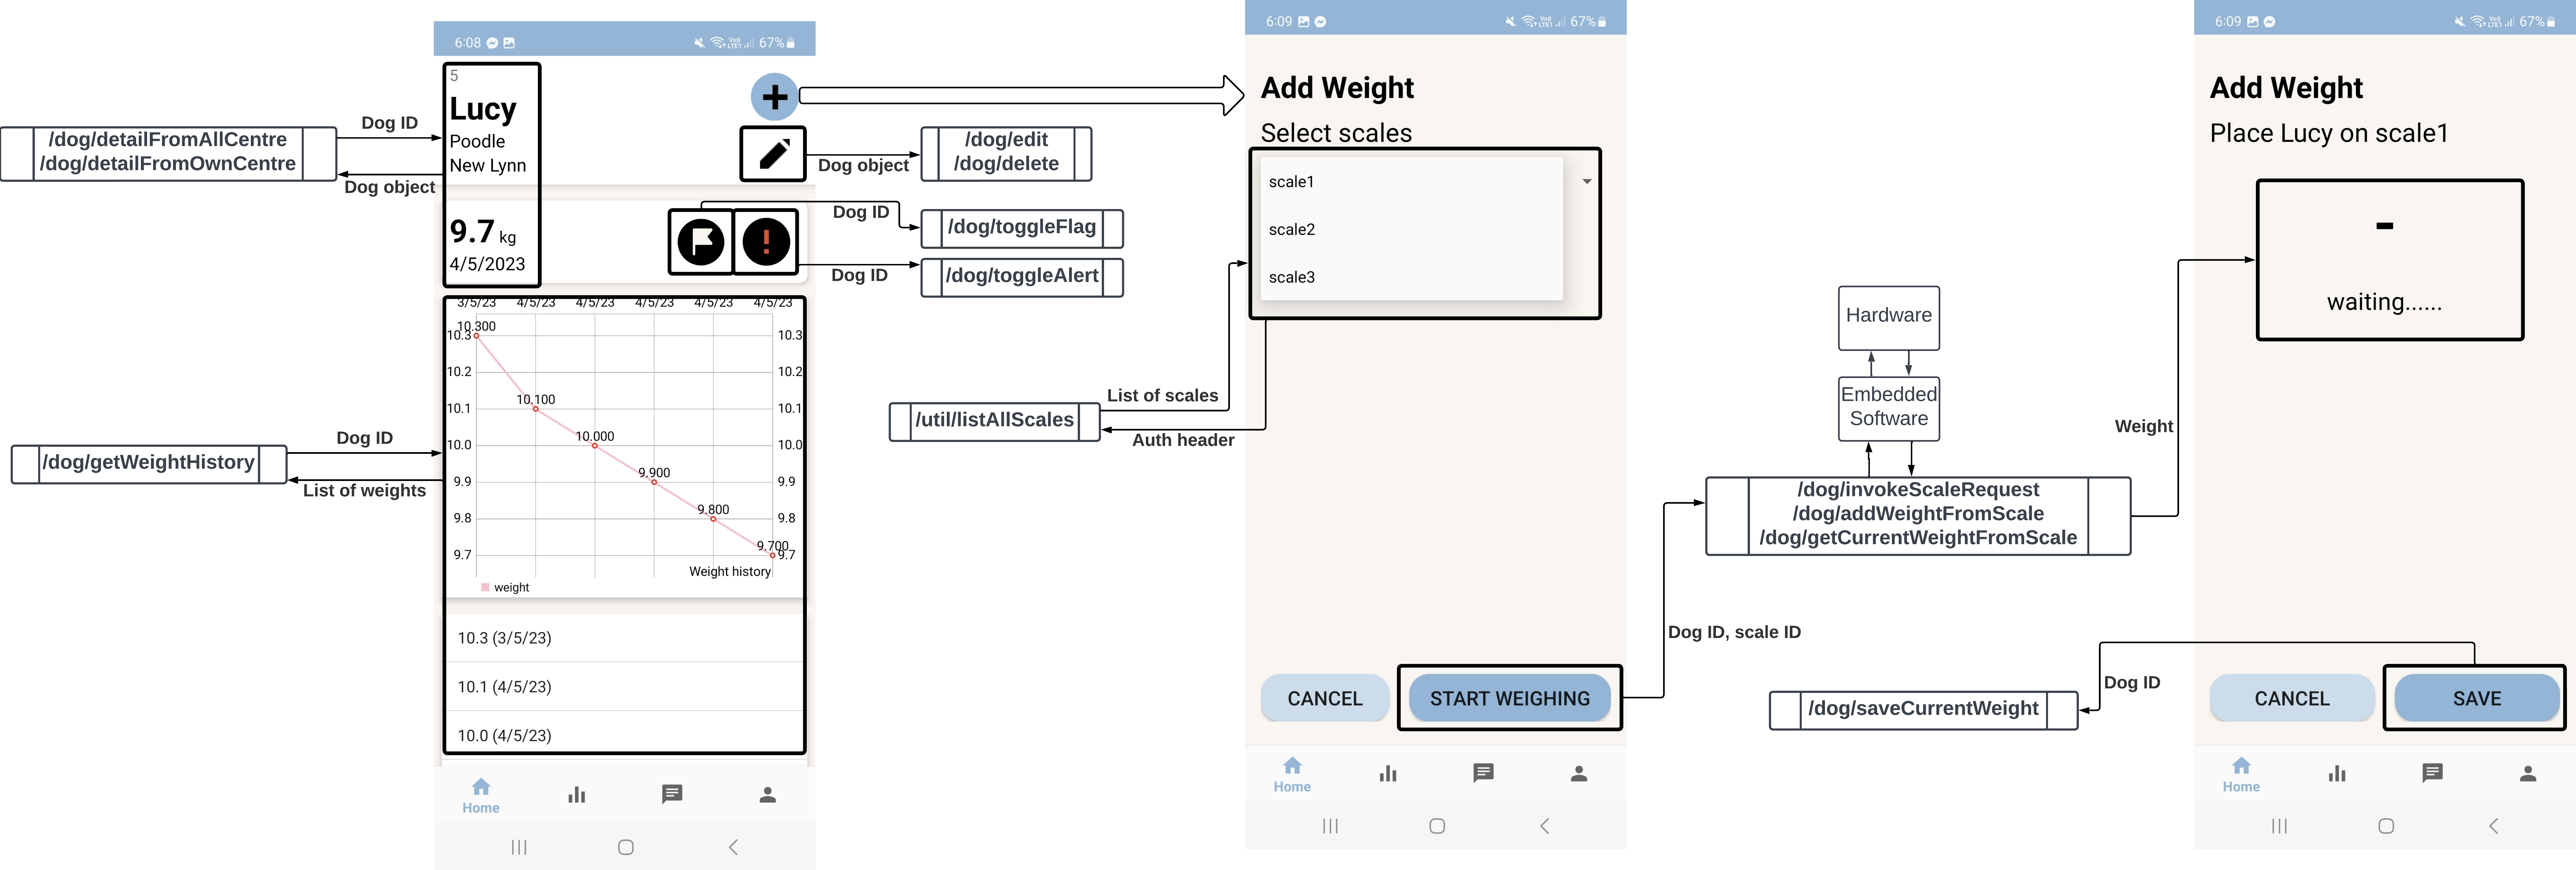
\includegraphics[scale=0.05]{dog_flow.png}
    \caption{Dog screen and data flow}
    \label{fig:mob_dog}
\end{figure}

\begin{figure}[!ht]
    \centering
    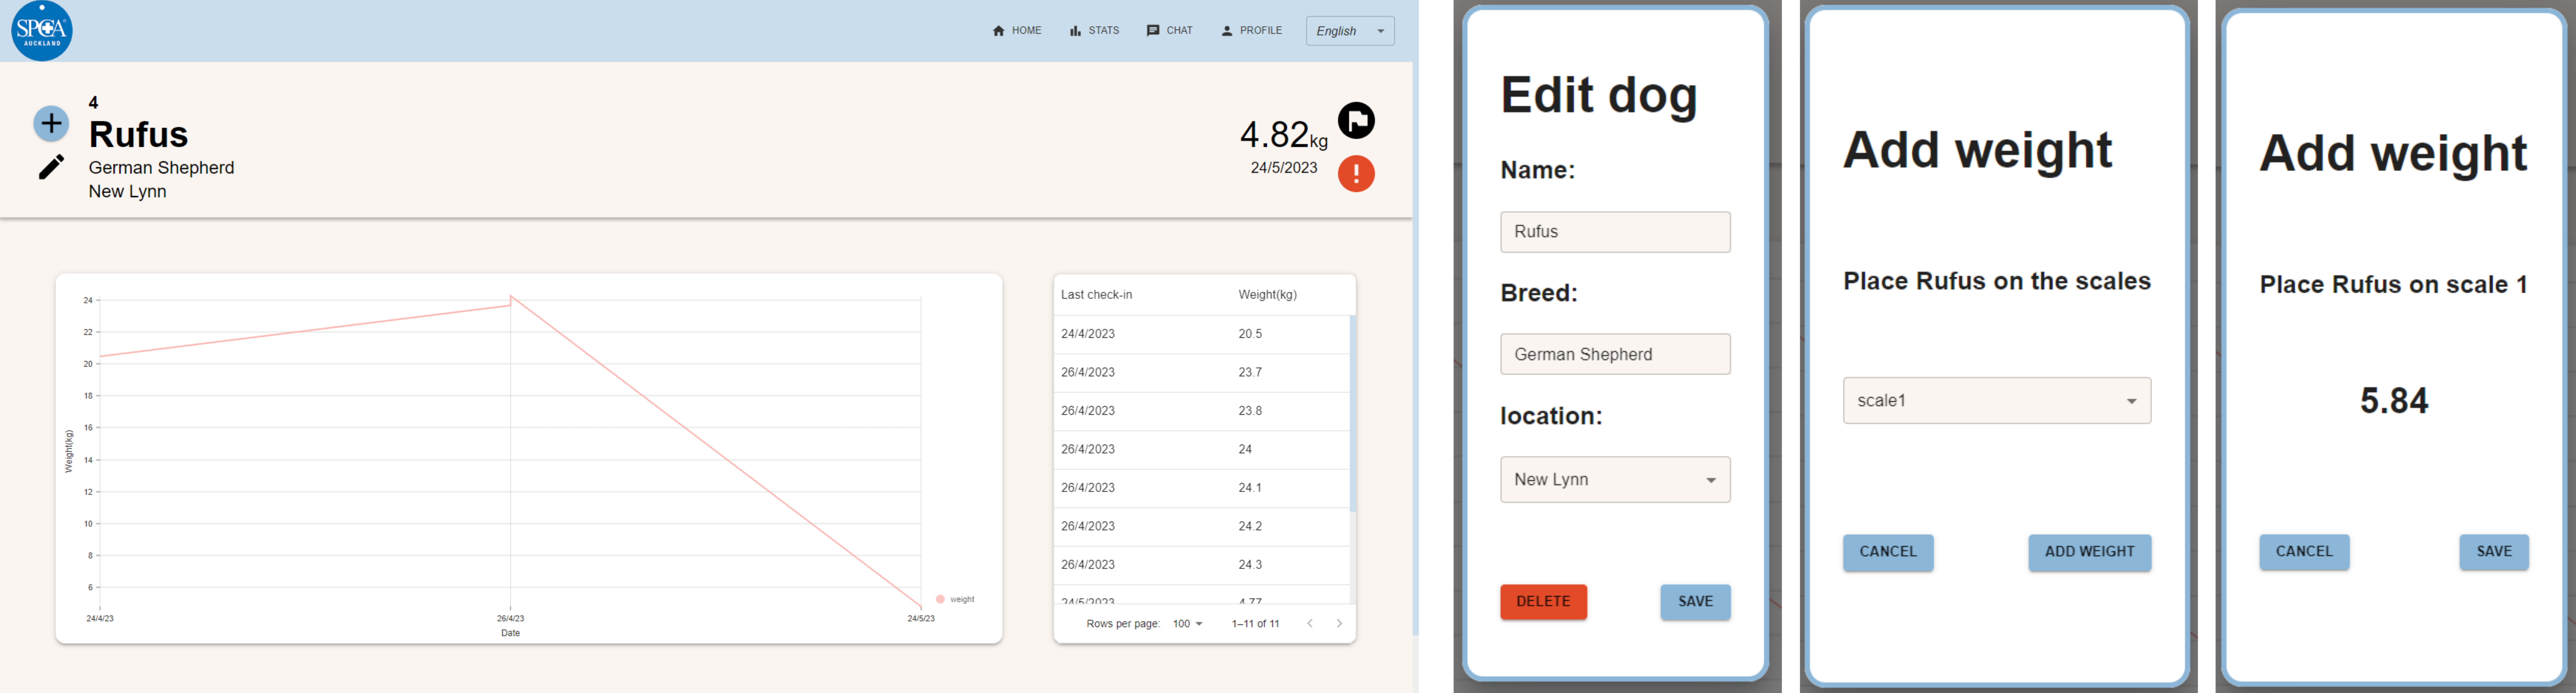
\includegraphics[scale=0.05]{dog_web.png}
    \caption{Web dog screen with additional pop-ups}
    \label{fig:web_dog}
\end{figure}

The statistics page, shown in figure \ref{fig:mob_stats}, allows the user to view data of their center, namely the weight distribution of all the dogs and the proportion of dogs weighed that week. This page will mostly be of use to administrators, but all users have access to the statistics of their centres. Seeing these statistics will allow them to check the overall health of the center 'at a glance', and administrators can view each center to identify any problems. Displaying the data in a visual representation surpasses any language barriers, and is easy for the user to understand.

\begin{figure}[!ht]
    \centering
    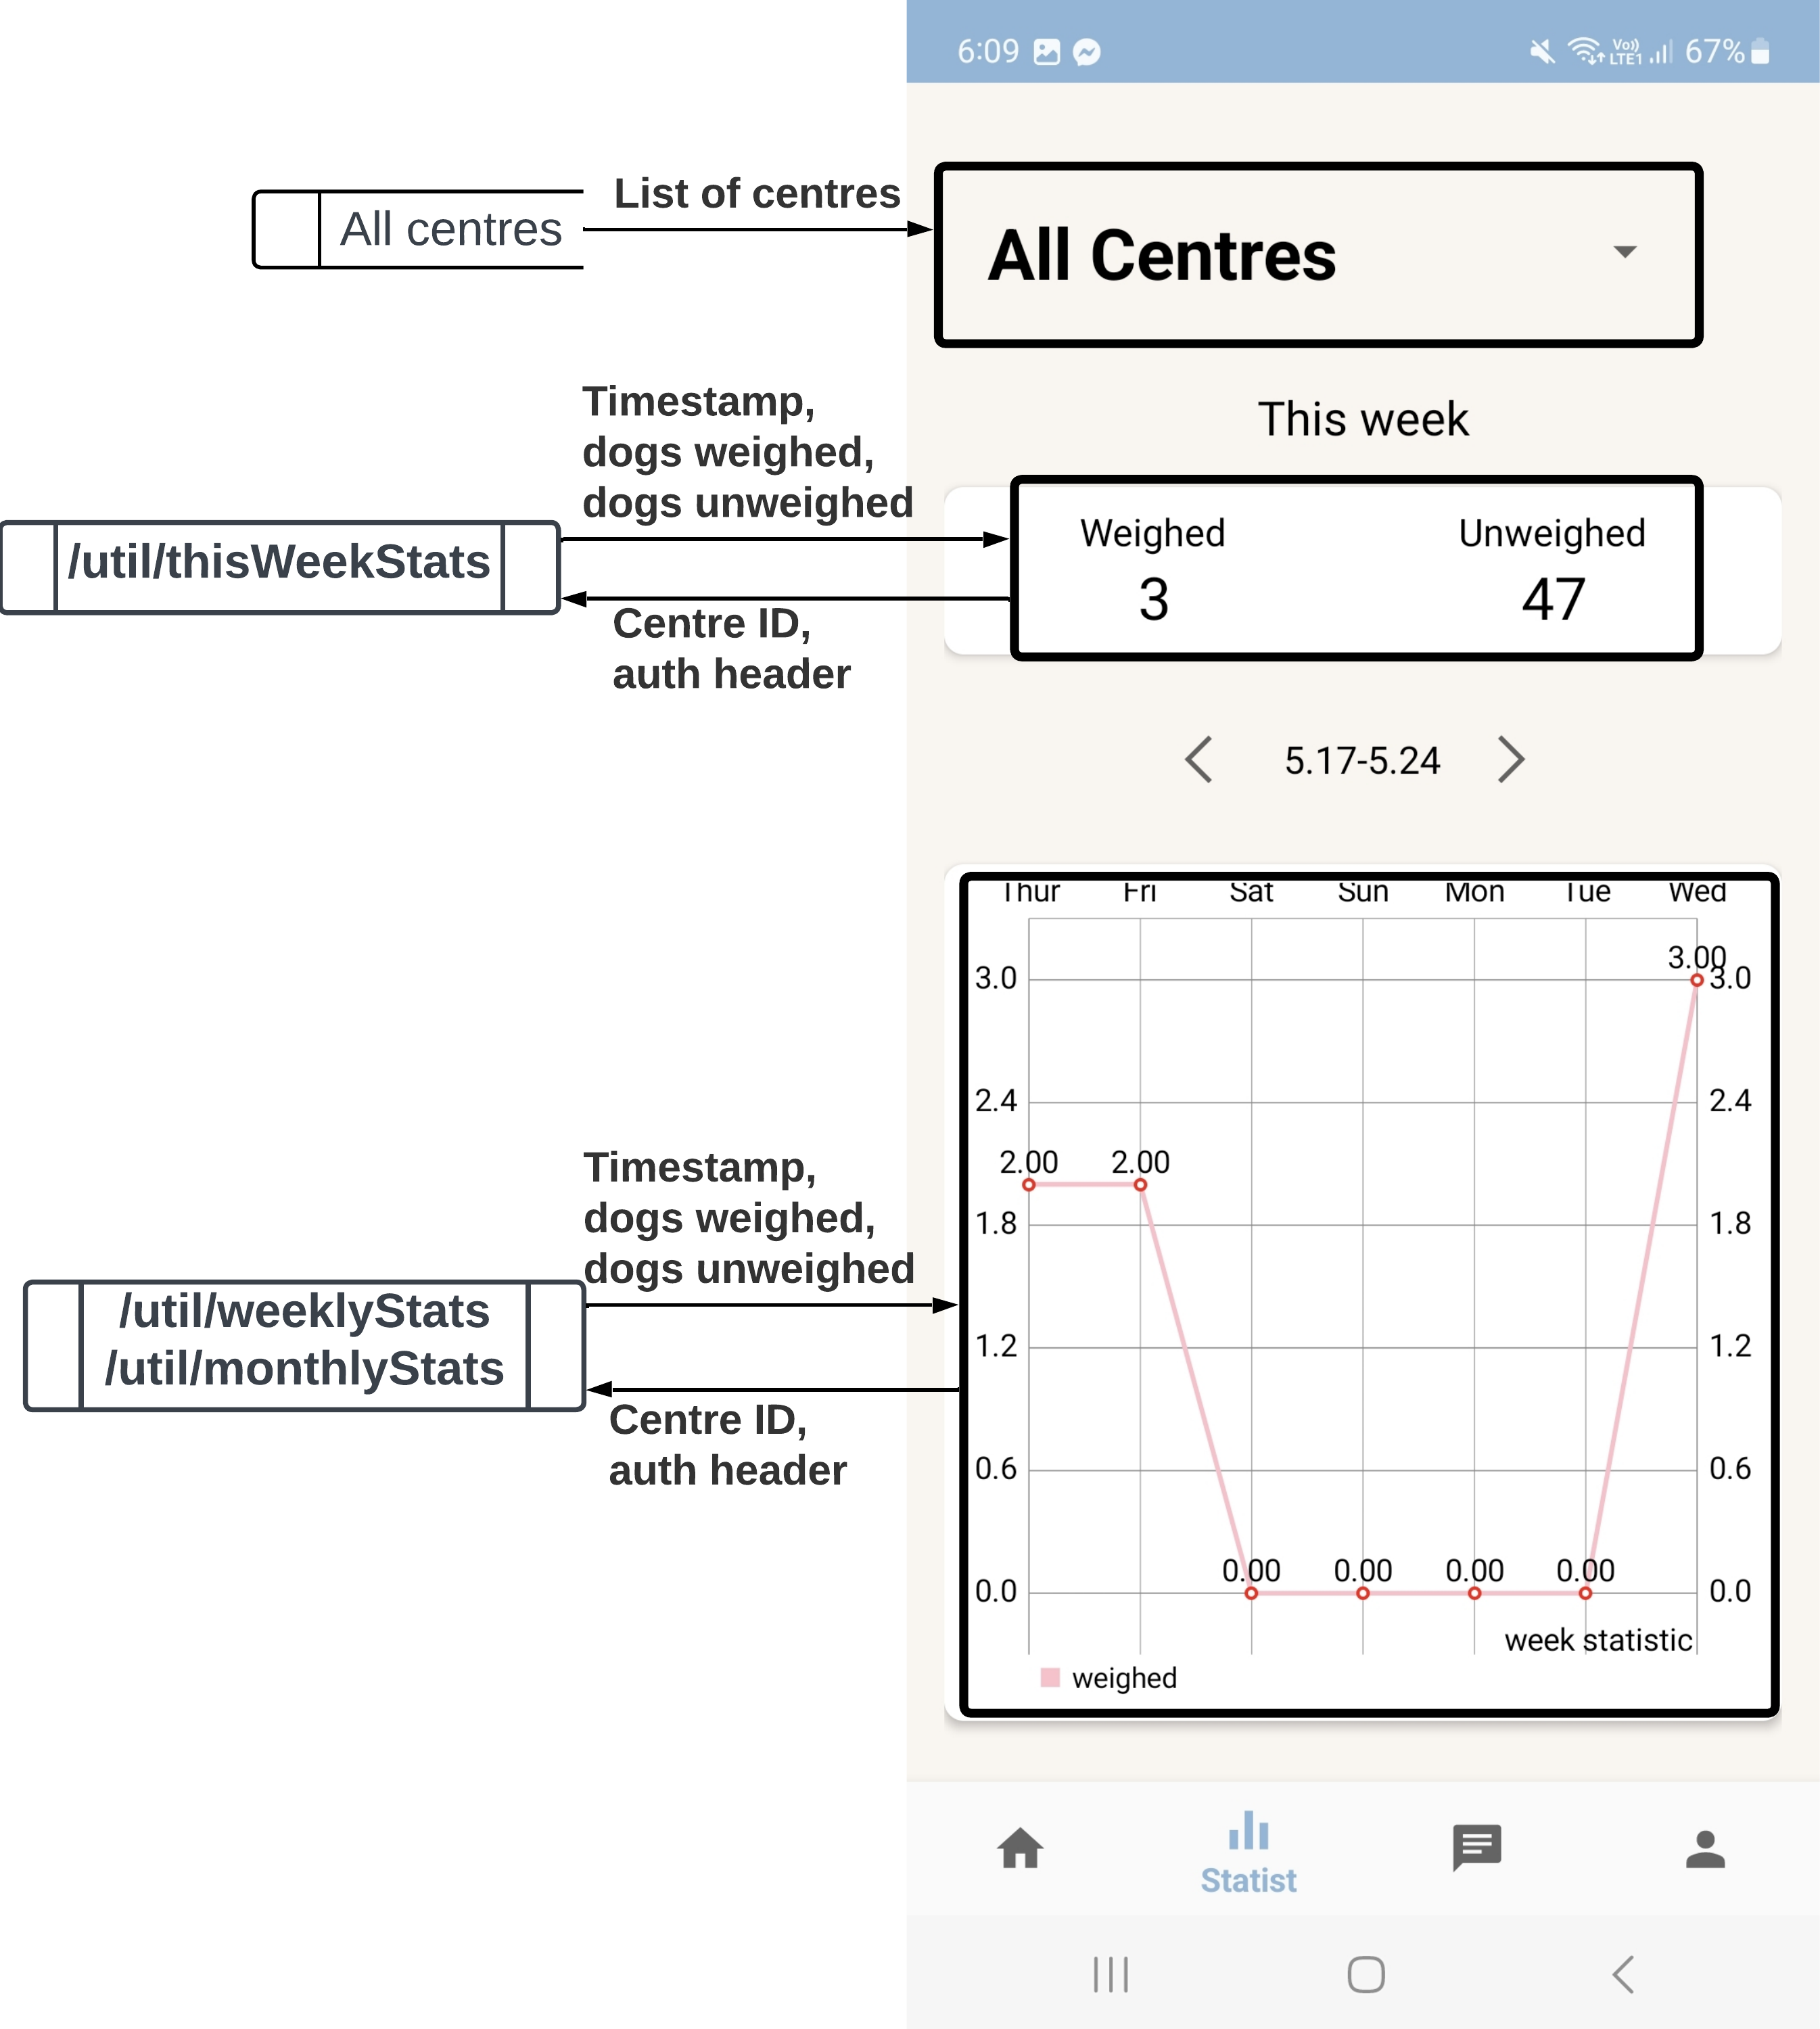
\includegraphics[scale=0.05]{stats_flow.png}
    \caption{Statistics screen and data flow}
    \label{fig:mob_stats}
\end{figure}

The chat page aims to foster whanaungatanga between SPCA staff, and improve their te taha whānau. The user can message anyone in the system, as seen in figure \ref{fig:mob_chat}, and therefore build connections. This will benefit the dogs' health as vets can talk to others and share their expertise, and it will benefit administrators by making it easier for them to communicate with others and complete their work. 

\begin{figure}[!ht]
    \centering
    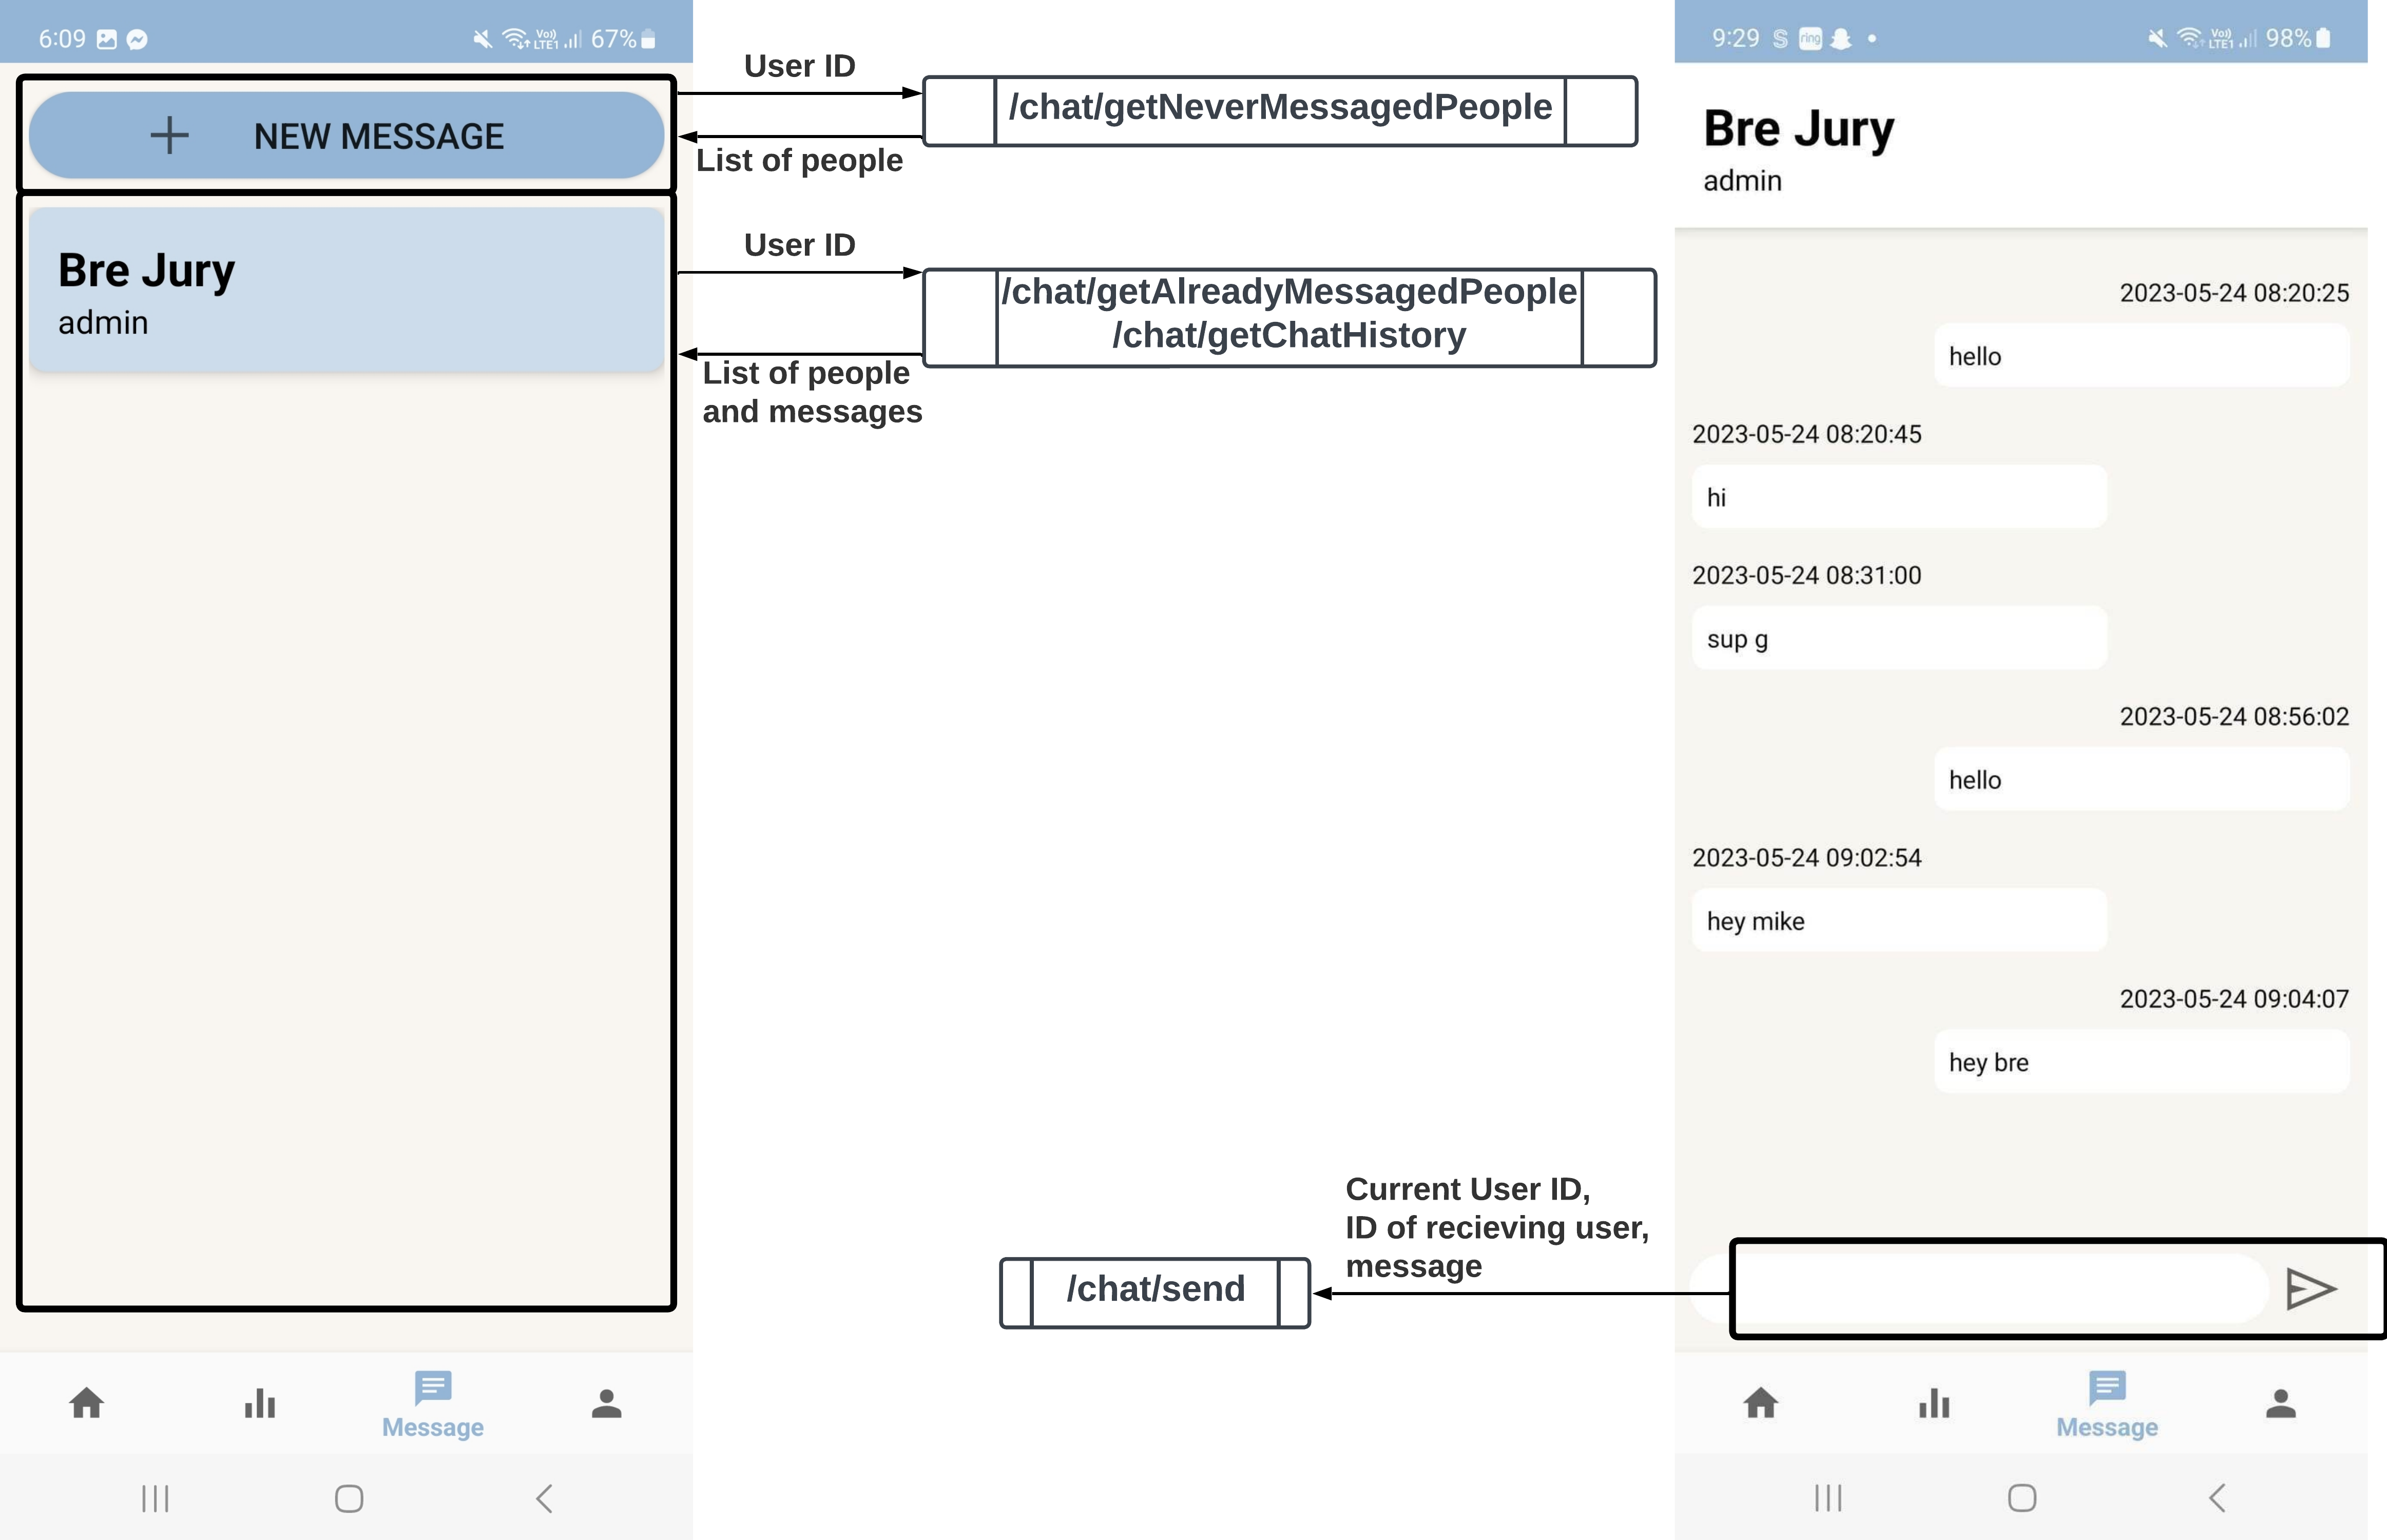
\includegraphics[scale=0.3]{chat_flow.png}
    \caption{Chat screen and data flow}
    \label{fig:mob_chat}
\end{figure}

The profile page shows their user their information, and allows them to change their password or log out, as shown in figure \ref{fig:mob_profile}. Admin users can also view the user management screen. This privilege isn't given to all users to protect the data and privacy of the staff. This screen allows administrators to edit existing users or add new users, and data can also be exported for any additional analytics the user may wish to perform. 

\begin{figure}[!ht]
    \centering
    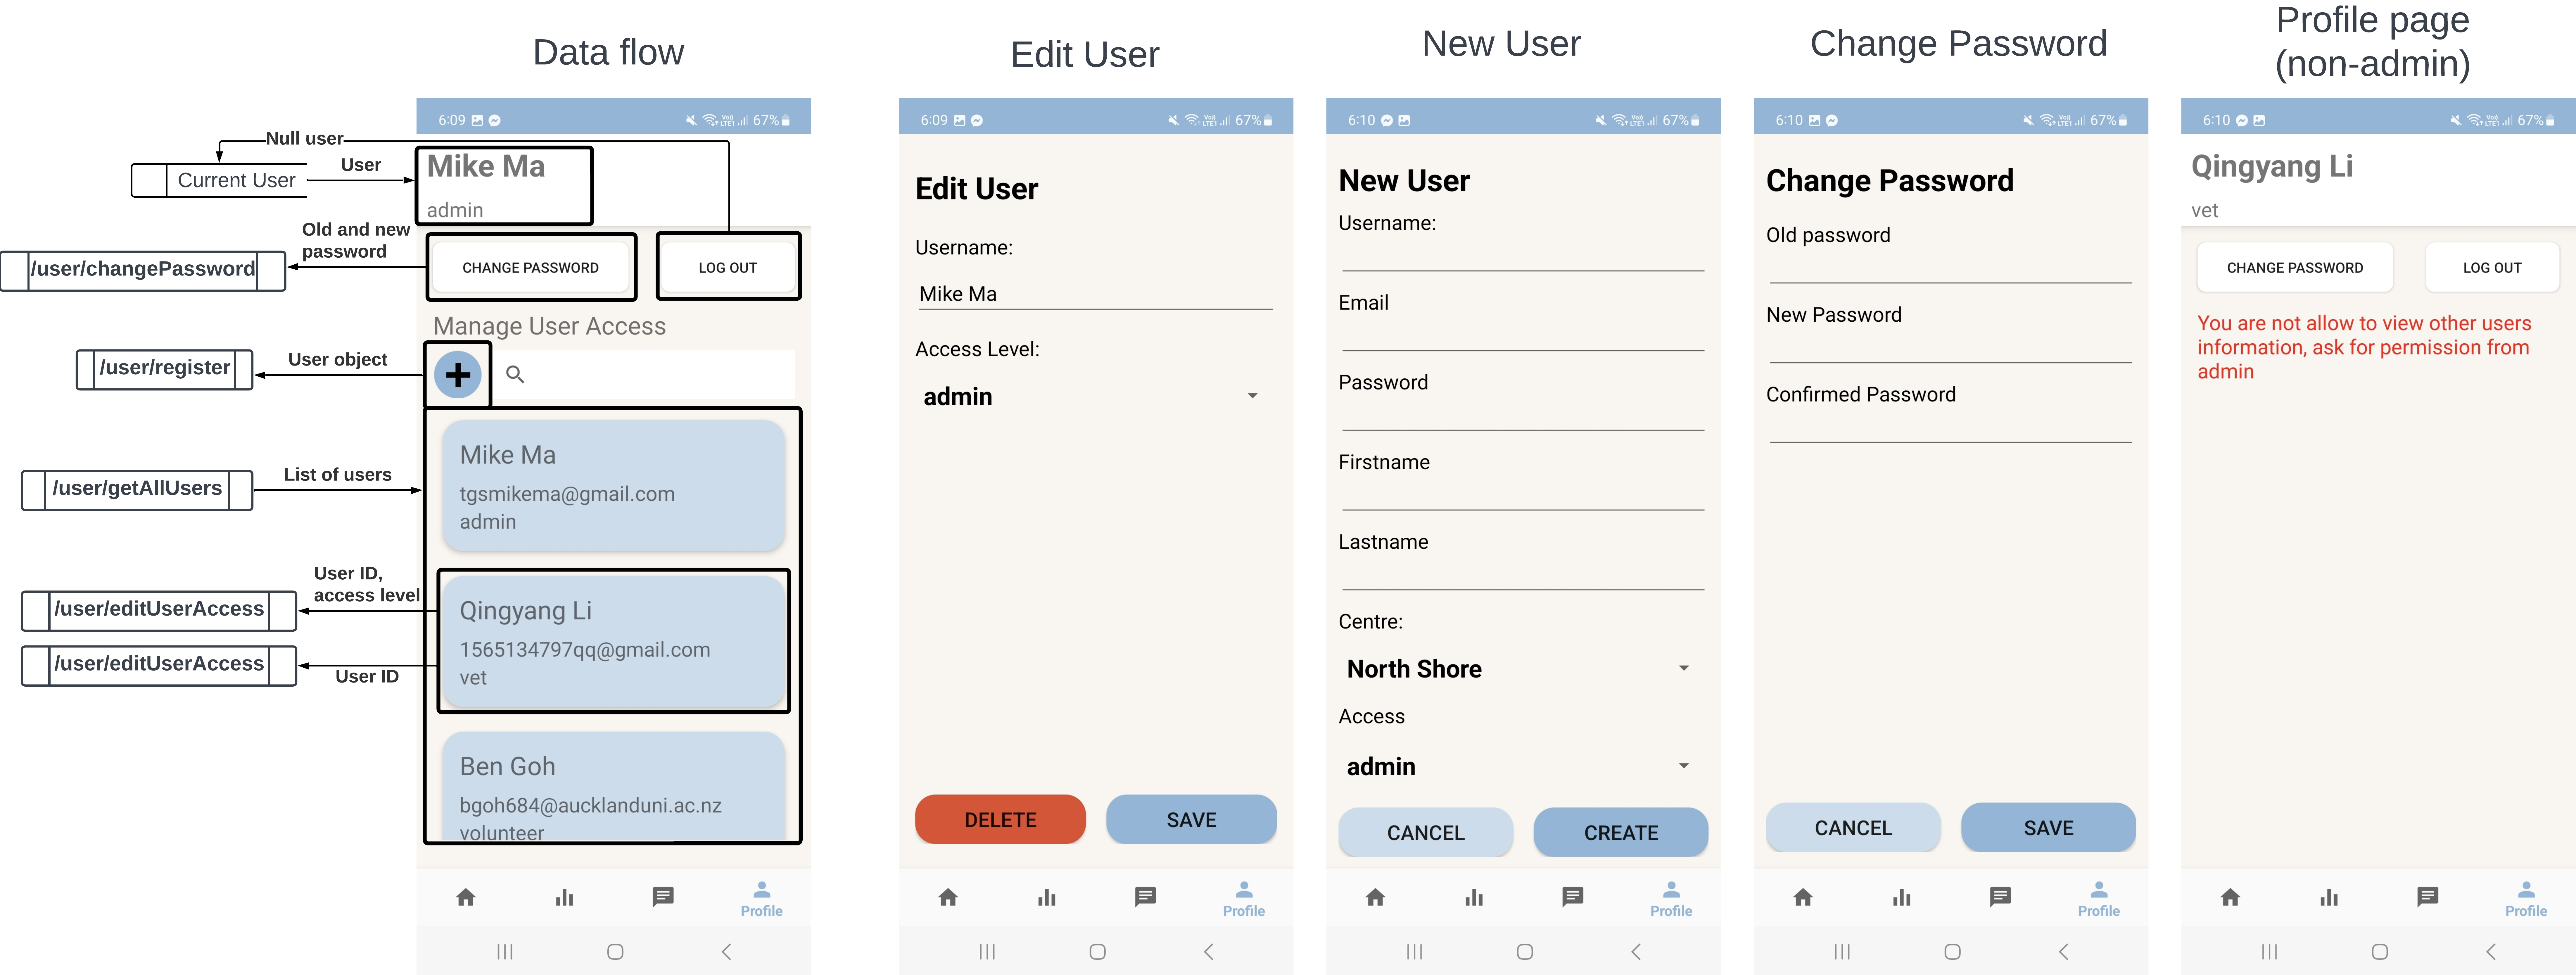
\includegraphics[scale=0.05]{profile_flow.png}
    \caption{Profile screen with additional pop-up screens and data flow}
    \label{fig:mob_profile}
\end{figure}

\section{Requirements Complicance}

\subsection{Concurrency}

There is no case where two different scales will weigh the same dog simultaneously, and there should be no case where the same scale weighs two dogs concurrently. However, two or more scales may send requests to the database simultaneously. The backend system can handle concurrent requests from more than 40 scales since the dog weight information from the scales is sent so that no two scales’ POST requests will interfere. Concurrent POST requests are handled using scale and dog identifiers within each POST request and a temporary request object to the database. The scale and dog identifiers correspond to specific scales and dogs found in the database. The temporary request object prevents concurrency issues for a dog if the connection between the scale and the application unexpectedly closes or if the user chooses not to save the weight measured. The frontend must confirm the weight measurement, which causes the temporary request object to permanently store a dog’s weight in the database. Thus, if the connection drops between the scale and the application, the weight saved in the temporary request object will be overwritten upon the subsequent weight measurement for that dog. The database deletes unconfirmed temporary requests within two seconds. This method prevents incomplete weight measurements from competing with actual measurements in the database.


\subsection{Data Storage Requirements}

The backend system meets the three months storage requirement as the SQLite database does not automatically reset. Through authentication, users can access all the information they are authorised to retrieve within the specified three-month requirement.

We use SQLite for our database. The database size of 30 staff and 50 dogs, including messages, scales, and temporary requests, is 53248 bytes. The maximum database size for SQLite is 281 terabytes, roughly 5.3 billion times larger than the current database size [2]. Thus, our backend system will store the data for 100 staff and 200 dogs.


